% AI-generated: this document was written and checked by TraceableAI (Department of Business Development and Technology, Aarhus University) with the language model fake-model.
% The method, counts, figures and references are written in code from the run's files; the prose is model
% text whose citations were checked against their sources. It has not been peer reviewed.
% Source code: https://github.com/lauPhilip/au-btech-literature-review-agent
% ----------------------------------------------------------------------------
% main.tex: Grey literature review (Garousi et al. (2019)) written by TraceableAI.
% Title: Context engineering: a grey literature review
% Run: RUN; tool: TOOL.
% Generated: DATE. This file is generated; it is not written by hand.
%
% How it was made: the method, the counts, the figures, the tables and the reference list were
% written in code from the run's files. A language model wrote the prose (title, abstract,
% introduction, results and discussion), and every citation in it was checked against the source
% it cites (citation-audit.json in the run's archive). All text from sources and from the model is
% escaped, so none of it can run a LaTeX command.
%
% Compile with pdflatex, twice for the cross-references (Overleaf does this for you). Every
% package is in TeX Live. Text has one sentence per line; LaTeX reads a line break as a space.
% The references are typeset at the end in the tool's APA 7 form. references.bib in the archive
% holds the same works under the same keys, so every \cite keeps working if you replace the
% thebibliography environment with \bibliographystyle{...} and \bibliography{references}.
%
% Fonts: TeX Gyre Termes for text, TeX Gyre Heros for sans serif and TeX Gyre Cursor for code. Where
% Aarhus University's AU Passata package (AUPassata.sty) is installed, it sets the sans serif text
% instead. AU Passata belongs to Aarhus University and is not shipped with this file; staff and
% students can install it from https://math.medarbejdere.au.dk/latex/au-fonts-for-latex
% ----------------------------------------------------------------------------

\documentclass[10pt,a4paper]{article}

%% Encoding and fonts
\usepackage[T1]{fontenc}
\usepackage[utf8]{inputenc}
\usepackage{tgtermes}
\IfFileExists{AUPassata.sty}{\usepackage{AUPassata}}{\usepackage{tgheros}} % AU Passata only where installed
\usepackage{tgcursor}
\usepackage{microtype} % fewer badly spaced lines in the narrow columns

%% Page layout: 20 mm on every side, the page number inside the bottom margin
\usepackage[a4paper,margin=20mm,includefoot]{geometry}
\usepackage{multicol}
\usepackage{fancyhdr}
\pagestyle{fancy}
\fancyhf{}
\renewcommand{\headrulewidth}{0pt}
\fancyfoot[C]{\sffamily\scriptsize\color{greyText} Page \thepage}
\setlength{\emergencystretch}{2em} % last resort for a line that cannot be filled

%% Maths
\usepackage{amsmath,amssymb}

%% Tables: booktabs rules; tabularx tables that may run over pages (ltablex)
\usepackage{booktabs}
\usepackage{ltablex}
\usepackage{capt-of} % a caption for a table set inside the two columns
\newcolumntype{Y}{>{\raggedright\arraybackslash}X}
\newcolumntype{L}[1]{>{\raggedright\arraybackslash}p{\dimexpr#1\linewidth-6pt\relax}}
\setlength{\LTcapwidth}{\textwidth}
\counterwithin{table}{section} % Table 4.1 is the first table of section 4

%% Figures, drawn with TikZ and pgfplots
\usepackage{xcolor}
\usepackage{float}
\usepackage{adjustbox}
\usepackage{pgfplots}
\usepgfplotslibrary{statistics}
\pgfplotsset{compat=1.18}
\usetikzlibrary{matrix,arrows.meta,positioning}
\definecolor{auBlue}{HTML}{003B5C}
\definecolor{greyText}{HTML}{4B5563}
\definecolor{customIndigo}{HTML}{312E81}

%% Citations, links and the PDF's metadata (hyperref comes last)
\usepackage{cite} % sorts and ranges the numbers: [1--4]
\usepackage{xurl} % a web address may break anywhere
\usepackage[hidelinks]{hyperref}
\hypersetup{
    pdftitle={Context engineering: a grey literature review},
    pdfauthor={TraceableAI (AI system), Department of Business Development and Technology, Aarhus University},
    pdfsubject={AI-generated literature review: written and checked by TraceableAI (Department of Business Development and Technology, Aarhus University) with the language model fake-model. It has not been peer reviewed.},
    pdfkeywords={AI-generated, literature review, TraceableAI, fake-model},
    pdfcreator={TraceableAI (Department of Business Development and Technology, Aarhus University) with the language model fake-model},
    pdfproducer={TraceableAI (AI-generated) with pdfLaTeX}
}
\urlstyle{same} % links in the text face, as APA sets them

\begin{document}

\begin{center}
  {\sffamily\bfseries\scriptsize\color{gray} AI-GENERATED GREY LITERATURE REVIEW\par}
  \vspace{4pt}
  {\rmfamily\LARGE\bfseries Context engineering: a grey literature review\par}
  \vspace{8pt}
  {\large TraceableAI – artificial researcher\textsuperscript{*}\par}
  \vspace{4pt}
  {\sffamily\small\color{greyText} Author names, affiliations and ORCID iDs (0000-{}0000-{}0000-{}0000): to be completed by the authors\par}
  \vspace{4pt}
  {\ttfamily\scriptsize\color{gray} Protocol fingerprint: FINGERPRINT \textbar{} Generated: DATE\par}
\end{center}
{\footnotesize\noindent\textsuperscript{*}An AI system; the person who planned the review is responsible for its use. A literature review written and checked by TraceableAI\@. It has not been peer reviewed.\par}
{\color{lightgray}\hrule}

\begin{abstract}
One source keeps running summaries.
\end{abstract}
\noindent{\small\textbf{Keywords:} context engineering for LLM agents; summaries keep the context short\par}
\vspace{12pt}

\begin{multicols}{2}

\section{Introduction}\label{sec:introduction}

\subsection{Rationale}\label{sec:rationale}

Agents keep a running summary~\cite{ana2025managing}.

\subsection{Objectives}\label{sec:objectives}

The review set out to answer five research questions: (RQ1) Which context engineering practices do practitioners and researchers describe?; (RQ1.1) Which tools and frameworks support these practices?; (RQ1.2) How are the practices usually applied when an agent is built?; (RQ2) How often is each practice mentioned in grey and in academic sources?; (RQ3) Is the use of retrieval for context related to fewer reported agent failures?

\section{Methodology}\label{sec:methodology}

\subsection{Planning (G1–G5)}\label{sec:planning-g1-g5}

The review's goal was: Map the practices that developers and researchers use to decide what goes into the context window of an LLM agent, and how they judge whether a practice works.
It was written for researchers and practitioners.
Whether to include grey literature was decided with the seven questions of the guidelines' Table 4 (G3): 6 of 7 were answered ``yes''.
The protocol was written on DATE (UTC), before any search, and its SHA-256 fingerprint is recorded with the plan (G1).

\par\smallskip\noindent{\scriptsize\setlength{\tabcolsep}{3pt}%
\noindent\begin{tabular}{@{}L{0.333}L{0.333}L{0.333}@{}}
  \toprule
  \textbf{Question} & \textbf{Text} & \textbf{Type (G5)} \\
  \midrule
\end{tabular}\par\nointerlineskip\nobreak%
\noindent\begin{tabular}{@{}L{0.333}L{0.333}L{0.333}@{}}
  RQ1 & Which context engineering practices do practitioners and researchers describe? & Description and classification \\
\end{tabular}\par\nointerlineskip%
\noindent\begin{tabular}{@{}L{0.333}L{0.333}L{0.333}@{}}
  RQ1.1 & Which tools and frameworks support these practices? & Existence \\
\end{tabular}\par\nointerlineskip%
\noindent\begin{tabular}{@{}L{0.333}L{0.333}L{0.333}@{}}
  RQ1.2 & How are the practices usually applied when an agent is built? & Descriptive process \\
\end{tabular}\par\nointerlineskip%
\noindent\begin{tabular}{@{}L{0.333}L{0.333}L{0.333}@{}}
  RQ2 & How often is each practice mentioned in grey and in academic sources? & Frequency distribution \\
\end{tabular}\par\nointerlineskip%
\noindent\begin{tabular}{@{}L{0.333}L{0.333}L{0.333}@{}}
  RQ3 & Is the use of retrieval for context related to fewer reported agent failures? & Relationship \\
\end{tabular}\par\nointerlineskip%
\noindent\begin{tabular}{@{}L{0.333}L{0.333}L{0.333}@{}} \bottomrule \end{tabular}\par
}\par\smallskip

\subsection{Search (G6–G8)}\label{sec:search-g6-g8}

The protocol named white papers and technical reports; product and project documentation; blog posts and practitioner articles; questions and answers on Q\&A sites; and code repositories and their README files as the kinds of grey literature to cover (G6); the sources the searches found were blog posts and practitioner articles.
On DATE (UTC), 1 search ran across 1 source with 1 search string (``context engineering'') and found 2 sources (G7).
Each raw answer was saved as received, with its SHA-256 fingerprint.
Stopping rule (G8): Effort bounded: the top 20 hits of each search string.

\par\smallskip\noindent{\scriptsize\setlength{\tabcolsep}{3pt}%
\noindent\begin{tabular}{@{}L{0.25}L{0.25}L{0.25}L{0.25}@{}}
  \toprule
  \textbf{Source} & \textbf{Search string} & \textbf{Returned} & \textbf{New} \\
  \midrule
\end{tabular}\par\nointerlineskip\nobreak%
\noindent\begin{tabular}{@{}L{0.25}L{0.25}L{0.25}L{0.25}@{}}
  Stack Exchange sites (Stack Overflow and others) & context engineering & 2 & 2 \\
\end{tabular}\par\nointerlineskip%
\noindent\begin{tabular}{@{}L{0.25}L{0.25}L{0.25}L{0.25}@{}} \bottomrule \end{tabular}\par
}\par\smallskip
Not done, and why:

\begin{itemize}
\item No general web search engine was used: none offers a search API that is free and allows its results to be kept, which a traceable review needs.
\item Practitioners and authors were not contacted for sources; only sources found by the searches were reviewed.
\end{itemize}

\subsection{Selection (G9, G10)}\label{sec:selection-g9-g10}

Each of the 2 sources found was screened once by the language model against the protocol's criteria (G9, G10).
Following the rapid-review practice of single screening with a verified sample, a source was screened a second time, independently and with the steps in a different order, when the first screening included it, was unsure (low or medium confidence, or no summary to judge by) or found text that looked like instructions to the model, and when it fell in a random audit sample of 20\% of its pool (at least 10), drawn with the seed SEED from every source the first screening decided, whatever it decided.
Of the 2 sources screened, 2 were screened twice and 0 once: 2 for a reason above (2 included, 0 unsure, 0 flagged), of which 2 agreed with the first screening, and 2 in the audit sample, 0 of them for that reason alone.
Cohen's $\kappa$ was computed on the audit sample only, so the targeted second screenings do not enter it: $\kappa$ = 1.00 over 2 sources.
Both screenings are the same model at temperature 0, so $\kappa$ measures how stable the model's decisions are, not agreement between two people. 2 were included, 0 excluded and 0 set aside as duplicates of a source with the same title. 1 decision was flagged for the reviewer: 1 because the source's text looked like instructions to the model.
The reviewer looked at 0 decisions and changed 0; 1 of the flagged decisions was not looked at, 0 of them exclusions that stand as the model made them; the model's decision stays on file next to the reviewer's.

Inclusion criteria: Sources whose main subject is how the context of an LLM agent is built, selected or managed, meaning what goes into its context window and why.
A source must explain at least one such practice, or evaluate one, in enough detail that a developer could apply it.
Exclusion criteria: Sources that mention an agent's context only in passing; generic tutorials on retrieval-augmented generation or vector databases; release notes and changelogs; code repositories whose README does not explain a practice; marketing pages without technical content; sources only about the wording of prompts for single chat requests; sources not in English.

\subsection{Quality (G11)}\label{sec:quality-g11}

Every included source was scored on the 20 items of the quality checklist in the guidelines' Table 7, each 1, 0.5 or 0 points, with a threshold of 10 points.
The language model answered the items that need reading the source, and every point it gave rests on a quote found in the kept text of the source's page; the date, the impact and the outlet type were decided in code (impact: 0.5 point from 1 citations, 5 score, 1,000 views, 3 answers, 100 stars, 20 forks, 20 points, 10 comments; 1 point from 10 citations, 50 score, 10,000 views, 10 answers, 1,000 stars, 200 forks, 100 points, 50 comments). 1 sources passed, 0 scored below the threshold and 1 could not be assessed, most often because their page could not be read.

Of the sources that passed, 0 came from 1st-tier outlets, 0 from 2nd-tier and 1 from 3rd-tier outlets (checklist item 8.1); their mean score was 18 of 20 points.

\subsection{Systematic map and extraction (G12)}\label{sec:systematic-map-and-extraction-g12}

The language model proposed the attributes of the systematic map from the research questions, with values generalised over 1 source that passed the quality check.
The reviewer kept it as proposed, and version 1 was fixed before any source was extracted. 1 sources were extracted against it; every value rests on a quote found in the kept text of the source's page, and what a page does not state was recorded as not stated.
The kind of each source, whether it is grey or formal literature, its site, date and quality points were recorded in code.

\par\smallskip\noindent{\scriptsize\setlength{\tabcolsep}{3pt}%
\noindent\begin{tabular}{@{}L{0.333}L{0.333}L{0.333}@{}}
  \toprule
  \textbf{Attribute} & \textbf{Question} & \textbf{Values} \\
  \midrule
\end{tabular}\par\nointerlineskip\nobreak%
\noindent\begin{tabular}{@{}L{0.333}L{0.333}L{0.333}@{}}
  Practice & RQ1 & Retrieval, Summarisation, Other \\
\end{tabular}\par\nointerlineskip%
\noindent\begin{tabular}{@{}L{0.333}L{0.333}L{0.333}@{}} \bottomrule \end{tabular}\par
}\par\smallskip

\subsection{Synthesis (G13)}\label{sec:synthesis-g13}

Each extracted value with its quote became a finding; 1 finding remained after every quote was checked again against the kept page text, never the live page, and checked by the language model for whether it supports its value.
For each research question, the findings were grouped in code by attribute and value, the map's values serving as the first codes; the language model then named the themes, placed the values in them, and named the tensions between sources within a theme.
A second, independent placement of the values in the other order agreed with the first with Cohen's $\kappa$ = 1.00 for RQ1; it did not change the themes.
The review produced 1 theme.
What each theme rests on (how many sources, their outlet tiers and quality points, grey or formal literature) was counted in code, never by the model.

\end{multicols}

\section{Data and the flow of sources}\label{sec:data-and-the-flow-of-sources}

The searches found 2 grey sources.
After 0 duplicates were set aside, 2 were screened and 2 included; 1 of them passed the quality threshold of 10 points and 1 were extracted against the systematic map.

Figure~\ref{fig:flow} shows the flow of sources, Figures~\ref{fig:kinds} and~\ref{fig:quality} the extracted sources by kind and outlet tier and the quality scores, and Table~\ref{tab:map-counts} how many sources state each value of the map.

\begin{figure}[H]
\centering
\begin{adjustbox}{max width=\linewidth}
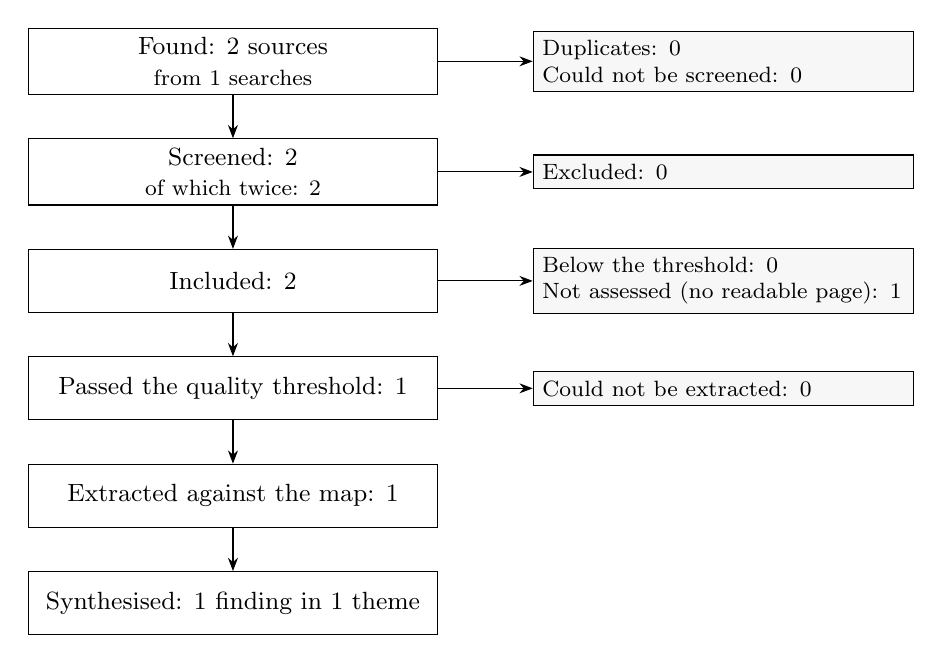
\begin{tikzpicture}[node distance=0.55cm and 1.2cm, box/.style={draw, rectangle, align=center, font=\small, minimum width=5.2cm, minimum height=0.8cm}, side/.style={draw, rectangle, align=left, font=\footnotesize, text width=4.6cm, fill=black!3}, >={Stealth}]
\node[box] (found) {Found: 2 sources\\{\footnotesize from 1 searches}};
\node[box, below=of found] (screened) {Screened: 2\\{\footnotesize of which twice: 2}};
\node[box, below=of screened] (included) {Included: 2};
\node[box, below=of included] (passed) {Passed the quality threshold: 1};
\node[box, below=of passed] (extracted) {Extracted against the map: 1};
\node[box, below=of extracted] (themes) {Synthesised: 1 finding in 1 theme};
\node[side, right=of found] (dup) {Duplicates: 0\\Could not be screened: 0};
\node[side, right=of screened] (exc) {Excluded: 0};
\node[side, right=of included] (low) {Below the threshold: 0\\Not assessed (no readable page): 1};
\node[side, right=of passed] (failed) {Could not be extracted: 0};
\draw[->] (found) -- (screened); \draw[->] (screened) -- (included); \draw[->] (included) -- (passed); \draw[->] (passed) -- (extracted); \draw[->] (extracted) -- (themes);
\draw[->] (found) -- (dup); \draw[->] (screened) -- (exc); \draw[->] (included) -- (low); \draw[->] (passed) -- (failed);
\end{tikzpicture}
\end{adjustbox}
\caption{Flow of sources from the searches to the synthesis}\label{fig:flow}
\end{figure}
\vspace{6pt}
\begin{figure}[H]
\centering
\begin{minipage}{0.48\textwidth}
\centering
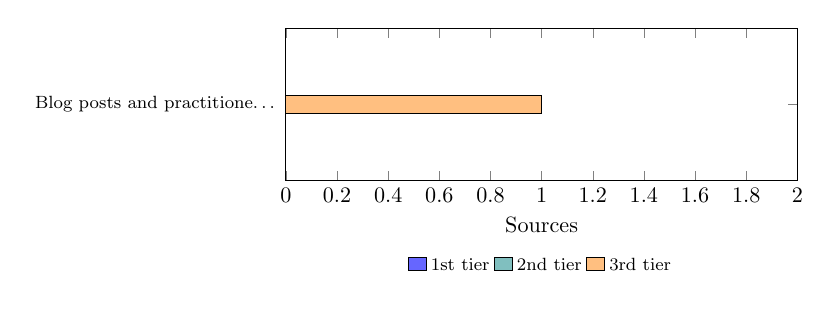
\begin{tikzpicture}[scale=0.8]
\begin{axis}[xbar stacked, ytick={1}, yticklabels={{Blog posts and practitione…}}, y dir=reverse, xmin=0, xmax=2, ymin=0.5, ymax=1.5, xlabel={Sources}, width=0.8\textwidth, height=4cm, bar width=8pt, yticklabel style={font=\footnotesize}, legend style={font=\footnotesize, at={(0.5,-0.45)}, anchor=north, legend columns=3, draw=none}]
\addplot[fill=blue!60] coordinates {(0,1)};
\addplot[fill=teal!50] coordinates {(0,1)};
\addplot[fill=orange!50] coordinates {(1,1)};
\legend{1st tier, 2nd tier, 3rd tier}
\end{axis}
\end{tikzpicture}
\caption{Extracted sources by kind (bar colour: outlet tier)}\label{fig:kinds}
\end{minipage}\hfill
\begin{minipage}{0.48\textwidth}
\centering
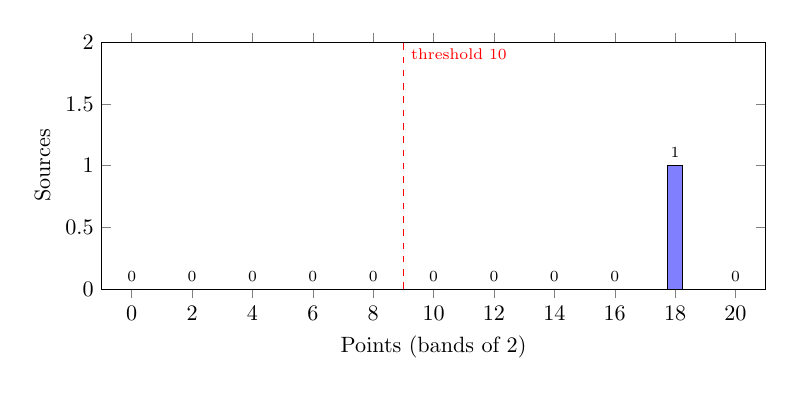
\begin{tikzpicture}[scale=0.8]
\begin{axis}[ybar, xtick={0,2,4,6,8,10,12,14,16,18,20}, xmin=-1, xmax=21, ymin=0, ymax=2, xlabel={Points (bands of 2)}, ylabel={Sources}, width=\textwidth, height=5.5cm, bar width=7pt, nodes near coords, every node near coord/.append style={font=\scriptsize}]
\addplot[fill=blue!50] coordinates {(0,0) (2,0) (4,0) (6,0) (8,0) (10,0) (12,0) (14,0) (16,0) (18,1) (20,0)};
\draw[red, dashed] (axis cs:9,0) -- (axis cs:9,2) node[pos=0.95, right, font=\scriptsize] {threshold 10};
\end{axis}
\end{tikzpicture}
\caption{Quality scores of the assessed sources (Table 7 checklist)}\label{fig:quality}
\end{minipage}
\end{figure}
\vspace{6pt}
\small
\begin{tabularx}{\textwidth}{YYYY}
\caption{The systematic map as counts}\label{tab:map-counts}\\
\toprule
\textbf{Attribute} & \textbf{Question} & \textbf{Value} & \textbf{Sources} \\
\midrule
\endfirsthead%
\toprule
\textbf{Attribute} & \textbf{Question} & \textbf{Value} & \textbf{Sources} \\
\midrule
\endhead%
Practice & RQ1 & Summarisation & 1 \\
\bottomrule
\end{tabularx}
\vspace{4pt}\noindent\textit{Counted in code from the 1 extracted sources; a source with several values counts once for each, and only values whose quote was found in the kept page and judged to support the value count.}\par
\normalsize
\vspace{10pt}

\begin{multicols*}{2}

\section{Results}\label{sec:results}

The results answer each research question in turn.
The 1 theme section was written by the language model from the findings of its theme only, and every citation in it was checked against the kept page of the source it cites; the note under each theme, on what it rests on, and the answers to questions about frequency, existence or a relationship are counted in code.

\subsection{RQ1: Summaries keep the context short}\label{sec:rq1-summaries-keep-the-context-short}

Sources keep a running summary of the conversation~\cite{ana2025managing}.

\par\smallskip\noindent{\small\textit{What this theme rests on: 1 source~\cite{ana2025managing}, 0 from 1st-tier, 0 from 2nd-tier and 1 from 3rd-tier outlets, with a mean quality of 18 of 20 points (3rd-tier grey literature only).}\par}

\subsection{RQ1.1: Which tools and frameworks support these practices?}\label{sec:rq1-1-which-tools-and-frameworks-support}

This question asks whether something exists.
The systematic map has no attribute for it, so it is not answered here.

\subsection{RQ1.2: How are the practices usually applied when an agent is built?}\label{sec:rq1-2-how-are-the-practices-usually-appl}

No extracted source states anything this question asks about, so the review cannot answer it from these sources.

\subsection{RQ2: How often is each practice mentioned in grey and in academic sources?}\label{sec:rq2-how-often-is-each-practice-mentioned}

This question asks how often something occurs.
The systematic map has no attribute for it, so it is not answered here.

\subsection{RQ3: Is the use of retrieval for context related to fewer reported agent failures?}\label{sec:rq3-is-the-use-of-retrieval-for-context}

The systematic map has no attribute for this question, so the sources do not allow the relationship to be answered.

\section{Discussion}\label{sec:discussion}

\subsection{Answers to the research questions}\label{sec:answers-to-the-research-questions}

\noindent\textbf{RQ1. Which context engineering practices do practitioners and researchers describe?} Sources keep a running summary of the conversation~\cite{ana2025managing}.\par\smallskip
\noindent\textbf{RQ1.1. Which tools and frameworks support these practices?} The systematic map has no attribute for this question, so the review does not answer it.\par\smallskip
\noindent\textbf{RQ1.2. How are the practices usually applied when an agent is built?} No extracted source states anything this question asks about, so the review cannot answer it from these sources.\par\smallskip
\noindent\textbf{RQ2. How often is each practice mentioned in grey and in academic sources?} The systematic map has no attribute for this question, so the review does not answer it.\par\smallskip
\noindent\textbf{RQ3. Is the use of retrieval for context related to fewer reported agent failures?} The systematic map has no attribute for this question, so the sources do not allow the relationship to be answered.\par\smallskip

\subsection{Interpretation}\label{sec:interpretation}

Running summaries keep agent contexts short~\cite{ana2025managing}.

\subsection{Limitations of the evidence}\label{sec:limitations-of-the-evidence}

The evidence rests on blog posts and documentation that are not peer reviewed.

\subsection{Limitations of the review}\label{sec:limitations-of-the-review}

A language model screened the sources, scored their quality, proposed the systematic map, extracted the values, formed the themes and wrote the text; every value and citation counts only with a quote found in the kept text, but the model's judgements were not all checked by a human reviewer.
The grey sources are not peer reviewed, and each was read as its page was kept on the access date; a page may have changed since.

\subsection{Implications for practitioners}\label{sec:implications-for-practitioners}

Practitioners can keep a running summary of the conversation~\cite{ana2025managing}.

\subsection{Implications for researchers}\label{sec:implications-for-researchers}

Comparative studies of summaries and retrieval in agents are missing from the theme on short contexts.

\subsection{Automated citation check}\label{sec:automated-citation-check}

An automated check compared the part of each cited sentence attributed to a source with the text of that source's page as it was kept on the access date.
Of 8 citations checked, 8 were judged supported, 0 partly supported and 0 not supported; 0 could not be verified, most often because the model's quote was not found word for word in the kept text, or because a source's kept text was missing or had changed.
A supporting verdict counts only when its quote is found verbatim in the kept text.
Every verdict, with the quoted evidence, is listed in citation-audit.\allowbreak{}json; these are model judgements and should be spot-checked by a human reviewer.

\section{Summary for practitioners}\label{sec:summary-for-practitioners}

For developers.
\begin{itemize}
\item Keep a running summary~\cite{ana2025managing}.
\item Summarise old turns~\cite{ana2025managing}.
\item Keep the summary short~\cite{ana2025managing}.
\end{itemize}

\section{Conclusion}\label{sec:conclusion}

Short contexts are the shared practice, and the evidence for them is thin.

\section{Declarations}\label{sec:declarations}

\subsection{Use of artificial intelligence}\label{sec:use-of-artificial-intelligence}

This review was conducted with TraceableAI (version VERSION), an open-source tool, following the multivocal literature review guidelines of Garousi et~al.\ (2019), with the large language model fake-model, in MONTH (run RUNID).
The protocol was written by the authors and fingerprinted before the search.
The model was used for screening the grey sources twice against the criteria, scoring their quality on the guidelines' checklist, proposing the systematic map, extracting each source's values, checking that each value's quote supports it, grouping the findings into themes, writing the theme sections, the answers to the research questions and the discussion, the limitations of the evidence, the implications and the conclusion, the summary for practitioners and the title, abstract and introduction, and checking each citation against the kept page of the source it cites.
Every value, quality point and citation verdict counts only with a quote found verbatim in the kept page text; the method, the counts, the figures, the answers to questions about frequency, existence or a relationship and the references were written in code.
On the random audit sample of 2 sources, the two screenings agreed with Cohen's kappa = 1.00; 2 of 2 targeted second screenings agreed with the first.
Both screenings were the same model at temperature 0, so kappa measures its stability, not agreement between people.
Screening decisions were not checked by a human reviewer within the tool.
The kept text of 1 of 1 source contained phrases addressed to a model as instructions; it was flagged for the reviewer and changed no decision.
The abstract and rationale were then given a language edit by the model into plain technical English (based on ASD-STE100).
Code kept an edit only when it changed no number, citation, quotation or technical name and left no sentence of more than 30 words; the text before and after each edit is on file.
The person who ran this review is responsible for checking this output and for how it is used.

\subsection{Registration and protocol}\label{sec:registration-and-protocol}

The review was not registered.
Its protocol (need and audience, the decision to include grey literature, research questions, kinds of grey literature, searches and search strings, stopping rule, criteria and quality threshold) was written on DATE (UTC), before any search; its SHA-256 fingerprint begins FINGERPRINT.
The file is part of the run archive.

\subsection{Availability}\label{sec:availability}

The code of the tool is openly available at \url{https://github.com/lauPhilip/au-btech-literature-review-agent}.
This run used a version of the tool.
The run archive contains the protocol, the raw search answers, every screening decision and quality score with its quotes, the systematic map, the extraction, the synthesis, the written paper, the citation audit and a manifest.json with the SHA-256 fingerprint of every file.
The kept page texts are fingerprinted but not redistributed.

\subsection{Support and funding}\label{sec:support-and-funding}

To be completed by the authors.

\subsection{Competing Interests}\label{sec:competing-interests}

To be completed by the authors.
Declare any financial or personal relationship that could be seen to influence the work, or state that there is none.

\subsection{Ethics Approval}\label{sec:ethics-approval}

Not required; the review involved no human participants and used only published or publicly available sources.

\subsection{Author Contributions}\label{sec:author-contributions}

To be completed by the authors.
Give each author's roles in the CRediT taxonomy, for example Conceptualization, Methodology, Investigation, Writing – original draft and Writing – review \& editing.

\end{multicols*}

\clearpage
\begin{thebibliography}{99}
\bibitem{ana2025managing} Ana (2025). Managing agent context.\ \textit{blog.\allowbreak{}example.\allowbreak{}org}.\ \url{https://blog.example.org/post} (accessed DATE; archived at \url{https://web.archive.org/web/TIMESTAMP/https://blog.example.org/post})
\end{thebibliography}

\clearpage
\section*{Appendix}\label{sec:appendix}
\setcounter{table}{0}
\renewcommand{\thetable}{A.\arabic{table}}
\renewcommand{\theHtable}{A.\arabic{table}} % hyperref's own name, so A.1 is not the same link as 0.1

\subsection*{Statements on the Use of AI for Submission}
Publishers ask for the use of AI to be disclosed in different places. Each statement below is written in code from the run's record; copy the one your venue asks for, check it and edit it to fit.
\paragraph{Declaration of generative AI and AI-assisted technologies in the manuscript preparation process}
\textit{Elsevier asks for this as a separate declaration before the references.} During the preparation of this work the authors used TraceableAI (version VERSION), an open-source review tool, with fake-model in order to screen sources, score their quality, propose the systematic map, extract and check values, group the findings into themes, write the paper's sections, check each citation against its source and edit the language of the abstract and rationale. The person who ran this review is responsible for checking this output and for how it is used.\par
\paragraph{Acknowledgments}
\textit{IEEE and ACM ask for the disclosure in the acknowledgements.} The search, screening, quality scoring, data extraction, a first draft of the paper and a language edit of the abstract and rationale were carried out with TraceableAI using fake-model; every citation was automatically checked against the kept text of the source it cites. The person who ran this review is responsible for checking this output and for how it is used.\par
\paragraph{Methods}
\textit{Springer Nature and Wiley ask for the disclosure in the methods section.} This review was conducted with TraceableAI (version VERSION), an open-source tool, following the multivocal literature review guidelines of Garousi et~al.\ (2019), with the large language model fake-model, in MONTH (run RUNID). The protocol was written by the authors and fingerprinted before the search. The model was used for screening the grey sources twice against the criteria, scoring their quality on the guidelines' checklist, proposing the systematic map, extracting each source's values, checking that each value's quote supports it, grouping the findings into themes, writing the theme sections, the answers to the research questions and the discussion, the limitations of the evidence, the implications and the conclusion, the summary for practitioners and the title, abstract and introduction, and checking each citation against the kept page of the source it cites. Every value, quality point and citation verdict counts only with a quote found verbatim in the kept page text; the method, the counts, the figures, the answers to questions about frequency, existence or a relationship and the references were written in code. On the random audit sample of 2 sources, the two screenings agreed with Cohen's kappa = 1.00; 2 of 2 targeted second screenings agreed with the first. Both screenings were the same model at temperature 0, so kappa measures its stability, not agreement between people. Screening decisions were not checked by a human reviewer within the tool. The kept text of 1 of 1 source contained phrases addressed to a model as instructions; it was flagged for the reviewer and changed no decision. The abstract and rationale were then given a language edit by the model into plain technical English (based on ASD-STE100). Code kept an edit only when it changed no number, citation, quotation or technical name and left no sentence of more than 30 words; the text before and after each edit is on file. The person who ran this review is responsible for checking this output and for how it is used.\par

\end{document}
